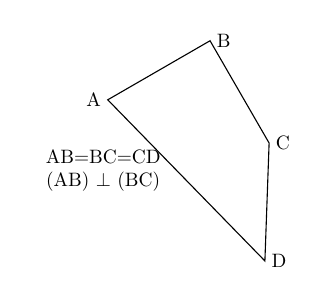
\begin{tikzpicture}[scale=0.5,every node/.style={scale=0.7},rotate=-60]

\draw (0,0) node [left]{A}--(0,3) node[right] {B}--(3,3) node[right] {C}--(5.54,1.41) node[right]{D}--cycle;
\node at(1.5,-1) {\begin{tabular}{c} AB=BC=CD \\ (AB) $\perp$ (BC) \end{tabular}};

\end{tikzpicture}